
\section{Extension to Mulitple Layers}
\subsection{Three Structures}
In this section, we introduce ways to extend the previous construction of adaptive wavelet tight frames to multiple layers. In going from one layer to multiple layers, we consider three typical structures which are conveniently illustrated in the following Figure.
\begin{center}
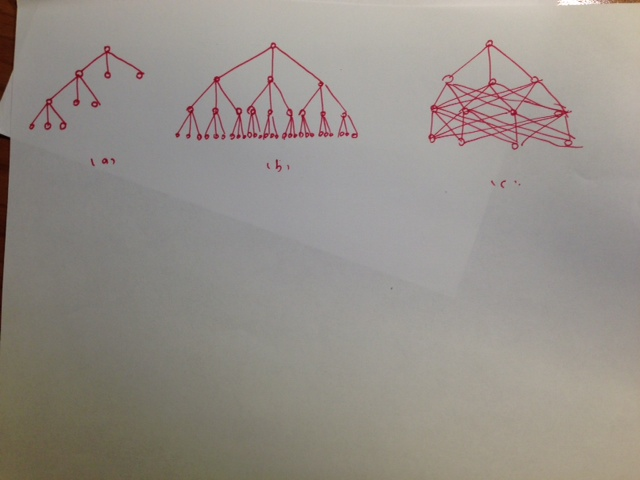
\includegraphics[scale=0.4]{arch.jpg}
\end{center}

The first structure is a partial $m-$tree, which corresponds to the multi-level wavelet or wavelet tight frame transform. The root node represents the input image, (for illustration purpose, the input image has only one channel), applying $m$ filters on the input, we get $m$ sets of wavelet tight frame coefficients. Each set of coefficients is represented using $m$-child nodes. The left most node always represents the low frequency coefficients. To do multi-level transform, we simply apply the same filters on the low frequency coefficients iteratively. Thus, for a level $L$ wavelet tight frame transform, the structure we get a tree of depth $L+1$ . 

This structure arises naturally in wavelet tight frames generated using MRA. The major advantage is the efficient decomposition and reconstruction algorithm. For level-$L$ transform with downsampling, it takes only $\mathcal O(mN)$ operations for the decomposition of a signal of length $N$.
 
Can we extend the previous adaptive construction to multiple levels using this structure? It depends. Such a structure assumes the existence of a single low frequency filter, which our previous construction does not guarantee. However, due to the pleasant surprise described in the previous section, for many datasets, we get a unique low frequency filter automatically. This phenomenon brings us a free lunch. It allows us to carry out multiple level transforms in exactly the same way as we do with pre-defined wavelet tight frames, only with improved performance. Our experience with numerical experiments suggests the rule of thumb, possibly exaggerated: {\color{red}wherever we have used wavelet tight frames for image processing tasks, we can try the adaptive construction using this structure. If we are lucky, we might improve the performance with no additional cost!} \\

The previous structure is great, but requires some luck. Sometimes we get a bunch of filters and no filter is more special than the others. This brings us to the second structure. The first layer is the same as the previous one. Below that, instead of doing transforms on the low frequency coefficients only, we do transforms on all sets of coefficients. As a result, the structure is a full $m$-tree. Apparently, the computational cost is now much larger. It is not appropriate for image compression or restoration tasks, but good for classification tasks. As the computational cost grows exponentially with the number of layers, we have to implement this structure with care and possibly some tricks in practice.  Examples of this structure include the scattering transform proposed by Mallat et.al. \\

It is the intention of creating a compact structure when we have no luck with the first structure that brings us to the third one. The first layer is still the same, below that, the tree structure is replaced by a fully connected structure. Because this structure is more elaborated and less known than the previous two, we shall give the details in the next subsection.

\subsection{The Proposed Multi-scale Structure}
The architecture consists an input layer and a few intermediate layers. The first layer is the same as the previous two structures, hence we focus on the intermediate layers. 

One intermediate layer accepts as input a few sets of coefficients produced by the previous layer, and produces another sets of output coefficients, not necessarily of the same number as the input. The input and output can be thought of as multi-channel images. The goal of the layer is still to produce sparse approximations of the input. Let $\{x_1,\cdots,x_m\}$ be the input coefficients, $\{v_1,\cdots,v_n\}$ be the output coefficients. The decomposition is defined as:
\begin{equation}
	v_j = \sum_i a_{ij}(-\cdot)*x_i,\quad j=1,\cdots,n
\end{equation}
and the reconstruction is defined as 
\begin{equation}
	x_i = \sum_j a_{ij}*v_j, \quad i=1,\cdots, m.
\end{equation}

Recognizing this as a 3D convolution, the UEP condition without downsampling then reads:
\begin{equation}
\label{uep:3d}
	\sum_{i=1}^m\sum_{j=1}^n  \sum_{n\in \mathbb{Z}^3} a_{ij}(k+n)a_{ij}(n) = \delta(k).
\end{equation}
We could explicitly incorporate this constraint and repeat what did in the previous sections. This amounts to solving
\begin{equation}
	\begin{aligned}
		&\min_{ \{a_{ij}\} } \sum_j \|v_j\|_1 \\
		\textrm{subject to} &\quad v_j = \sum_i a_{ij}(-\cdot)*x_i \\
			&\{a_{ij}\} \textrm{ satisfies \eqref{uep:3d}} \\
	\end{aligned}
\end{equation}
 But in practice, we find the resulting optimization program is not quite feasible to solve using a normal optimization procedure(It could be done though, just takes some time). Hence, we consider the following model based on the same sampling approximation spirit.
\begin{equation}
\label{eq:m3}
\begin{aligned}
	\min_{a_1,\cdots,a_m, v_1,\cdots,v_m}& \sum_i \|y_i - \sum_j a_{ij}*u_j\|_2 +\lambda \sum_j \|v_j\|_1 \\
	 \textrm{s.t.}  \quad v_j& = \sum_{i} a_{ij}(-\cdot)*x_i \\
		u_j&=\uparrow\downarrow(\sum_i a_{ij}(-\cdot)*y_i), \forall j.
	\end{aligned}
\end{equation}
The $\uparrow \downarrow$ represented a down-sampling followed by a up-sampling operation. It could be omitted if we are only interested in linear transform, however, the sampling operator need not be linear, it could be, for example max pooling and it reverse which are defined as 
\[
	\downarrow(c_1,\cdots,c_n) = (\arg\max_{c_1,\cdots,c_n} |c_i|, \arg\max_{i=1,\cdots,n} |c_i|)
\]
and its reverse
\[
	\uparrow(v,p)=(0,0,v,\cdots,0) \textrm{ with $v$ at the $p$-th location}.
\]
Unlike the linear sampling, in this case, we have to record both the value and position to get a reverse operation.

Similar to what did before, in the case where there is perturbation on the coefficients, we consider a particularly useful variant which we use in the numerical experiments.
\begin{equation}
\label{eq:m5}
\begin{aligned}
	\min_{\{a_{ij}\}, v_1,\cdots,v_m}& \sum_i \|y_i - \sum_j a_{ij}*u_j\|_2 +\lambda \sum_j \|v_j\|_1 + \eta \sum_j \|v_j-  \sum_{i} a_{ij}(-\cdot)*x_i \|_2^2\\
	 \textrm{s.t.}  	\quad 	u_j&=\uparrow\downarrow(\sum_i a_{ij}(-\cdot)*y_i), \forall j.
	\end{aligned}
\end{equation}
There is a subtlety considering stacking intermediate layer to form a multi-scale structures. That is, the output to input relation cannot be linear, otherwise stacking multiple layers would just be equivalent as a one layer structure. The non-linearity in our model may possibly come from two sources: one is the nonlinear sampling procedure, the other is the thresholding in the encoding stage.

Using \eqref{eq:m5} as a building block, we stack multiple layers together, we finally get the multi-scale structure depicted in Figure. The filters are all learned layer by layer, starting with the first one. Once the optimization has converged for the layer, we then move on to learn the next while keeping all filters in previous layers fixed.
